%%________________________________________________________________________
%% LEIM | PROJETO
%% 2022 / 2013 / 2012
%% Modelo para relat�rio
%% v04: altera��o ADEETC para DEETC; outros ajustes
%% v03: corre��o de gralhas
%% v02: inclui anexo sobre utiliza��o sistema controlo de vers�es
%% v01: original
%% PTS / MAR.2022 / MAI.2013 / 23.MAI.2012 (constru�do)
%%________________________________________________________________________


%%________________________________________________________________________
\chapter{Um Detalhe Adicional}
\label{ch:umDetalheAdicional}
%%________________________________________________________________________

Durante o processo de desenvolvimento deste projeto, foi utilizado um sistema de gest�o de vers�es para poder guardar todo o progresso do trabalho. Este sistema de gest�o perimitiu guardar e recuperar as v�rias vers�es que foram sendo desenvolvidas ao longo do trabalho realizado. Entre os v�rios documentos guardados nas vers�es salienta-se o relat�rio, c�digo desenvolvido e outras ideias ou rascunhos de �til an�lise. 

Foi utilizado o \textit{Git} para fazer a ineterliga��o entre o reposit�rio local e o reposit�rio na \textit{Internet}. O projeto foi realizado individualmente, por isso, foi apenas utilizado um ramo (\textit{branch}) no processo de gest�o de vers�es.


%%________________________________________________________________________
\chapter{Outro Detalhe Adicional}
\label{ch:outroDetalheAdicional}
%%________________________________________________________________________

\begin{figure}[h]
   \centering
   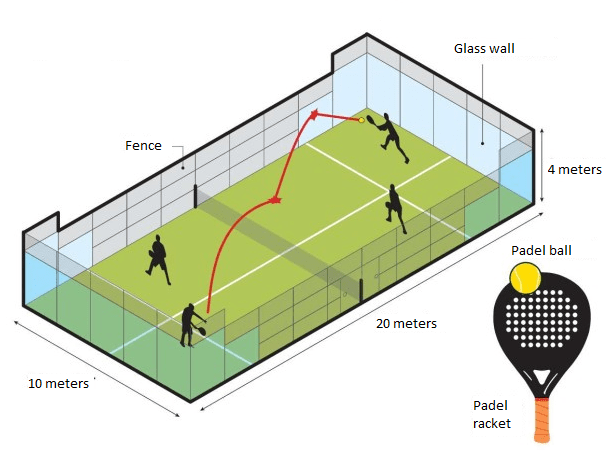
\includegraphics[width=10cm]{./padel_court}
\caption{Descri��o pormenorizada do campo de padel. \cite{tennisnerd_padel_2019}}
\label{fig:campopadel}
\end{figure}

\begin{figure}[h]
   \centering
   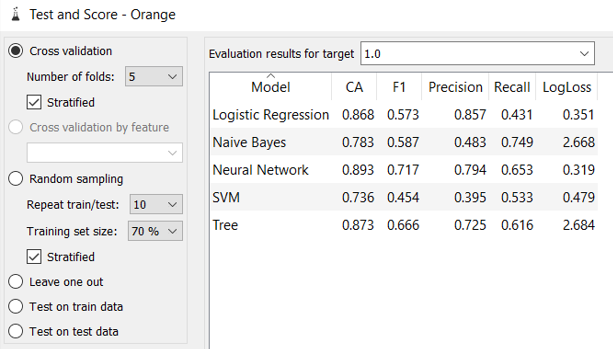
\includegraphics[width=12cm]{./positives_evaluation_0_5_1024}
\caption{Resultados da aplica��o de v�rios algoritmos aos dados para a classe dos positivos.}
\label{fig:odm_results_positives}
\end{figure}

\begin{figure}[h]
   \centering
   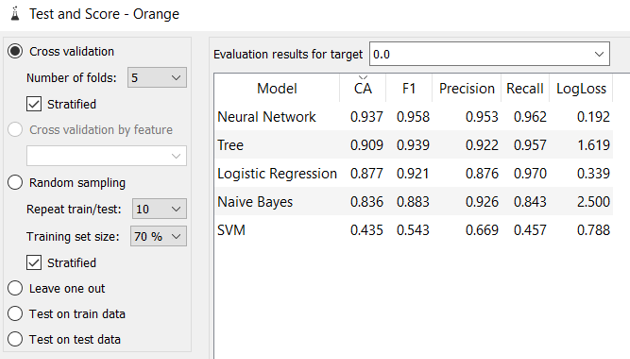
\includegraphics[width=12cm]{./negatives_evaluation_0_5_1024}
\caption{Resultados da aplica��o de v�rios algoritmos aos dados para a classe dos negativos.}
\label{fig:odm_results_negatives}
\end{figure}














